% Options for packages loaded elsewhere
\PassOptionsToPackage{unicode}{hyperref}
\PassOptionsToPackage{hyphens}{url}
%
\documentclass[10pt,a4paper]{article}
\usepackage[left=25mm,right=25mm]{geometry}
\usepackage{amsmath}
\usepackage{amsfonts}
\usepackage{amssymb}

\usepackage{amsmath,amssymb}
\usepackage{lmodern}
\usepackage{iftex}
\ifPDFTeX
  \usepackage[T1]{fontenc}
  \usepackage[utf8]{inputenc}
  \usepackage{textcomp} % provide euro and other symbols
\else % if luatex or xetex
  \usepackage{unicode-math}
  \defaultfontfeatures{Scale=MatchLowercase}
  \defaultfontfeatures[\rmfamily]{Ligatures=TeX,Scale=1}
\fi
% Use upquote if available, for straight quotes in verbatim environments
\IfFileExists{upquote.sty}{\usepackage{upquote}}{}
\IfFileExists{microtype.sty}{% use microtype if available
  \usepackage[]{microtype}
  \UseMicrotypeSet[protrusion]{basicmath} % disable protrusion for tt fonts
}{}
\makeatletter
\@ifundefined{KOMAClassName}{% if non-KOMA class
  \IfFileExists{parskip.sty}{%
    \usepackage{parskip}
  }{% else
    \setlength{\parindent}{0pt}
    \setlength{\parskip}{6pt plus 2pt minus 1pt}}
}{% if KOMA class
  \KOMAoptions{parskip=half}}
\makeatother
\usepackage{xcolor}
\usepackage{longtable,booktabs,array}
\usepackage{multirow}
\usepackage{calc} % for calculating minipage widths
% Correct order of tables after \paragraph or \subparagraph
\usepackage{etoolbox}
\makeatletter
\patchcmd\longtable{\par}{\if@noskipsec\mbox{}\fi\par}{}{}
\makeatother
% Allow footnotes in longtable head/foot
\IfFileExists{footnotehyper.sty}{\usepackage{footnotehyper}}{\usepackage{footnote}}
\makesavenoteenv{longtable}
\usepackage{graphicx}
\makeatletter
\def\maxwidth{\ifdim\Gin@nat@width>\linewidth\linewidth\else\Gin@nat@width\fi}
\def\maxheight{\ifdim\Gin@nat@height>\textheight\textheight\else\Gin@nat@height\fi}
\makeatother
% Scale images if necessary, so that they will not overflow the page
% margins by default, and it is still possible to overwrite the defaults
% using explicit options in \includegraphics[width, height, ...]{}
\setkeys{Gin}{width=\maxwidth,height=\maxheight,keepaspectratio}
% Set default figure placement to htbp
\makeatletter
\def\fps@figure{htbp}
\makeatother
\setlength{\emergencystretch}{3em} % prevent overfull lines
\providecommand{\tightlist}{%
  \setlength{\itemsep}{0pt}\setlength{\parskip}{0pt}}
\setcounter{secnumdepth}{-\maxdimen} % remove section numbering
\ifLuaTeX
  \usepackage{selnolig}  % disable illegal ligatures
\fi
\IfFileExists{bookmark.sty}{\usepackage{bookmark}}{\usepackage{hyperref}}
\IfFileExists{xurl.sty}{\usepackage{xurl}}{} % add URL line breaks if available
\urlstyle{same} % disable monospaced font for URLs
\hypersetup{
  hidelinks,
  pdfcreator={LaTeX via pandoc}}

\author{}
\date{}



\usepackage{listings}
\usepackage{color}

\definecolor{dkgreen}{rgb}{0,0.6,0}
\definecolor{gray}{rgb}{0.5,0.5,0.5}
\definecolor{mauve}{rgb}{0.58,0,0.82}

\lstset{frame=tb,
  language=C,
  aboveskip=3mm,
  belowskip=3mm,
  showstringspaces=false,
  columns=flexible,
  basicstyle={\small\ttfamily},
  numbers=none,
  numberstyle=\tiny\color{gray},
  keywordstyle=\color{blue},
  commentstyle=\color{dkgreen},
  stringstyle=\color{mauve},
  breaklines=true,
  breakatwhitespace=true,
  tabsize=3
}

\usepackage{multicol}
\usepackage{graphicx}
\usepackage{epstopdf}

\epstopdfDeclareGraphicsRule{.gif}{png}{.png}{convert gif:#1 png:\OutputFile}
\AppendGraphicsExtensions{.gif}
\usepackage{chngcntr}
\counterwithin*{equation}{section}
\counterwithin*{equation}{subsection}

\usepackage{float} 

\usepackage{amsmath}
\let\oldsubsection\subsection
\renewcommand{\subsection}{%
    \setcounter{equation}{0}%
    \oldsubsection%
}

\begin{document}


\begin{flushleft}
\begin{LARGE}CPRE 488 Homework 3 Spring 2024
\end{LARGE}
\\Digital Camera Sensor
\\Jonathan Hess
\\\href{https://github.com/Jetsama/CPRE488/tree/main/HW3}{GitHub Page}
\end{flushleft}

\section{Problem 1}
\begin{quote}
Decode the following I2C waveform, assuming the top signal is SDA and the bottom signal is SCL. What
transaction is being requested? Defend your answer.
\end{quote}

\begin{figure}[H]
\centering
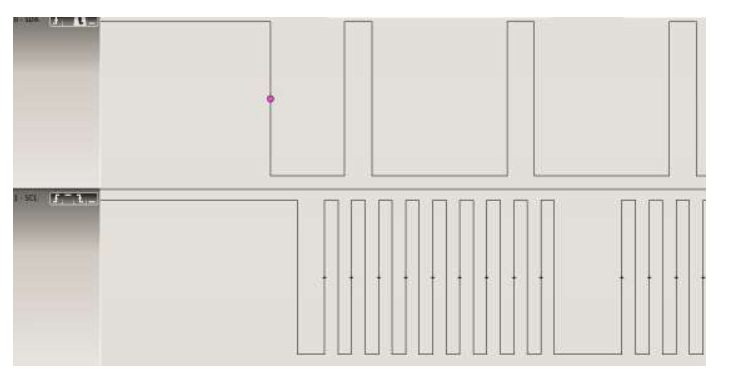
\includegraphics[width=5in]{images/Problem1.png} \\
\caption{The provided I2C signal}
\end{figure}
The first thing to examine is that the edge of the clock does not matter.
\begin{figure}[H]
\centering
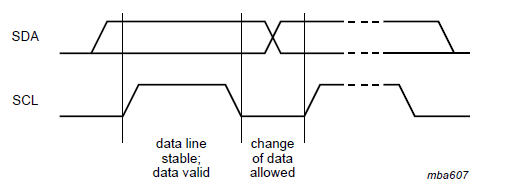
\includegraphics[width=5in]{images/i2c_bit_trnsf.jpg} \\
\caption{When data is set and read on an I2C signal\cite{jeremy}}
\end{figure}
This is because the change on the edges is illegal. Only when the clock is set low can the value be set.

Using this information we can get a binary value of signal.
\begin{figure}[H]
\centering
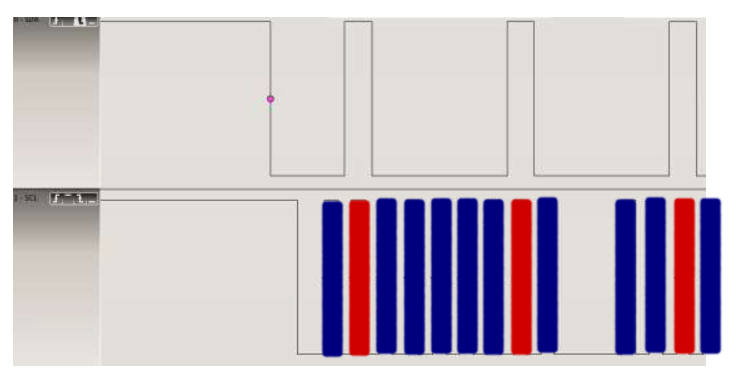
\includegraphics[width=5in]{images/Problem1-colored.png} \\
\caption{The colored I2C signal where red = 1 and blue = 0}
\end{figure}
The total binary value is 0b0100000100010. This can be broken up into the different frames.\\
I am making an assumption that this is at the beginning of the communication. This will need to be confirmed. This can be confirmed by the start of the signal where the SDA is pulled low before the SCL (normally not allowed). This is the signal for the start of the messaging.\\
The first frame is the 7 bit address. We know it is 7 bit and not 10 bit because the first bits of the signal are not 11110.\cite{spark}
ADDR is 0b0100000
The second frame is the read write bit which is 1 (the controller is requesting). \\
The next frame is the ACK with one bit. The bit tells if there was an error. It is 0.\\

What is concerning is that a lot of the images describing the protocol show the SDA returning high after acknowledgment. What I think is happening is that the responder is setting the SDA low immediately after acknowledgment (because it has to be ready for the clock signal).\\

\begin{figure}[H]
\centering
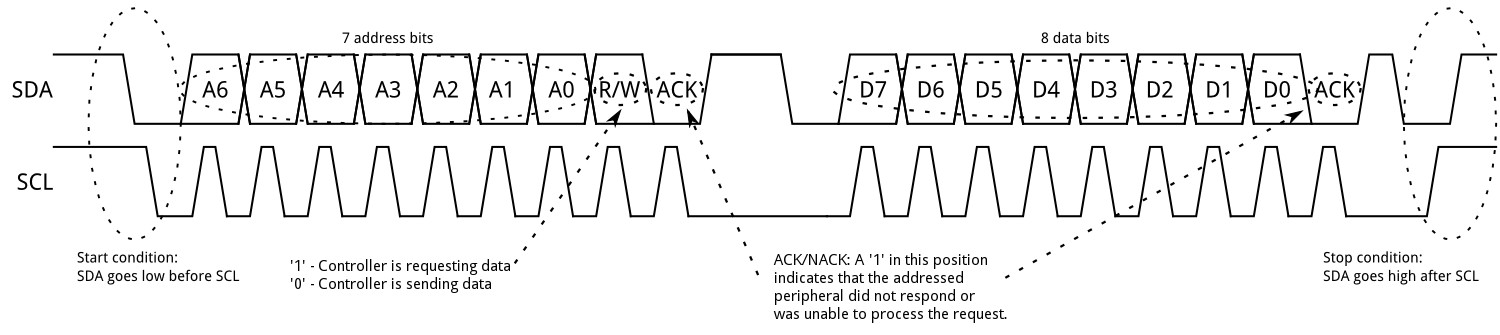
\includegraphics[width=5in]{images/I2C_Basic_Address_and_Data_Frames.jpg} \\
\caption{An example message with the I2C protocol with idle in between the address and data\cite{spark}}
\end{figure}


So we know that the controller is requesting data from a 7 bit addressable responder. It was a valid request because the aknowledge bit was set low and we even seen some of the data at the very end "0010...".
 
\section{Problem 2}
\begin{quote}
Fun with Documentation. Unlike in previous labs, where it was possible to get by without reading any of the
background material or documentation, the driver development in MP-3 will make you a very sad panda if you don’t have a good feel for embedded Linux.\\
\\For starters, Xilinx maintains a very nice wiki on porting Linux to Zynq-based devices. In MP-3, we will not be
following their directions precisely, but it provides a useful overview of several of the major steps involved. Read
through the wiki (starting here: http://www.wiki.xilinx.com/Getting+Started), and in your writeup, describe the
4 files that are needed to boot Linux on Zynq.\\
\end{quote}

\subsection{Problem 2a}\begin{quote}

The first file that you need is the image to put onto the SD card. This is what contains the OS.\\ 
They are avialable at the \href{https://xilinx-wiki.atlassian.net/wiki/spaces/A/pages/18842316/Linux+Prebuilt+Images}{Linux Prebuilt Images} page.\\
\end{quote}

The second file needed is the PetaLinux BSP. We are using the Zynq 7000 board which can be seen \href{https://www.xilinx.com/products/boards-and-kits/ek-z7-zc702-g.html}{here}. This means that we are using the \href{https://www.xilinx.com/member/forms/download/xef.html?filename=xilinx-zc702-v2019.2-final.bsp}{ZC702 PetaLinux BSP}.\\



\subsection{Problem 2b}\begin{quote}

\begin{quote}
Next, open up the Zynq-7000 technical reference manual, which is available on the CprE 488 course webpage:
http://class.ece.iastate.edu/cpre488/resources/ug585-Zynq-7000-TRM.pdf. Read all 1800+ pages (or just
Chapter 6, your choice) and provide a summary, in your own words, of the steps involved in the Zynq boot
process. Where does code get executed from, how does the programmable logic get programmed, etc.?\\


\\Finally, check out the Linux Device Drivers reference, also available on the course webpage:
http://class.ece.iastate.edu/cpre488/resources/ldd3.pdf. Specifically, focus on Chapters 1-3 and 13. In your
writeup, answer the following three questions:
\end{quote}

\subsection{Problem 2a}\begin{quote}

What are the three different classes of devices in Linux? Which class is most appropriate for a USB
missile launcher? Briefly defend your answer.
\end{quote}

\subsection{Problem 2b}\begin{quote}
From a programmer’s perspective, what makes driver development different from user-space
application development? For example, why can we not call libc functions such as printf()? Why is
floating-point code not allowed?
\end{quote}

\subsection{Problem 2c}\begin{quote}

What is the difference between major and minor device numbers? Does it matter which device number
we use for our missile launcher?
What is an “urb” in the context of a USB device drive
\end{quote}


\begin{thebibliography}{9}

\bibitem{jeremy}\href{https://jeremyclark.ca/wp/telecom/i2c-programming-scope-detection/}{I2C Programming \& Scope Detection}
\bibitem{spark}\href{https://learn.sparkfun.com/tutorials/i2c/all
}{I2C SparkFun}
\end{thebibliography}

\end{document}
